\documentclass[10pt,a4paper]{article}
	\usepackage[utf8]{inputenc}
	\usepackage{wrapfig}
	\usepackage{nameref}
	\usepackage{xcolor}
	\usepackage{colortbl}
	\usepackage{fancyhdr}
	\usepackage{cleveref}
	\usepackage{lastpage}
	\usepackage{tocloft}
	\usepackage{float}
	\usepackage{csquotes}
	\usepackage{titlesec}
	\usepackage{enumitem}
	\usepackage{subcaption}
	\usepackage[style=apa,natbib]{biblatex}
	\usepackage[pages=some]{background}
	\usepackage[hidelinks]{hyperref}
	\usepackage{titling}
	\usepackage{graphicx}
	\usepackage[margin=0.75in]{geometry}
	\usepackage[space]{grffile}
\graphicspath{ {screen captures/} }
\author{6273632 - mkem114}
\title{Papr $|$ SOFTENG 350 Assignment \# 3 Design Document}

\begin{document}
	\definecolor{orangeBack}{RGB}{51, 122, 183}
	\pagestyle{fancy}
	\fancyhf{}
	\renewcommand{\headrulewidth}{5pt}
	\renewcommand{\headrule}{\hbox to\headwidth{%
	  \color{orangeBack}\leaders\hrule height \headrulewidth\hfill}}
	\renewcommand{\footrulewidth}{5pt}
	\renewcommand{\footrule}{\hbox to\headwidth{%
	  \color{orangeBack}\leaders\hrule height \footrulewidth\hfill}}
	\renewcommand{\cftsecleader}{\cftdotfill{\cftdotsep}}
	\lfoot{\theauthor}
	\chead{Papr $|$ SOFTENG 350 Assignment \# 3 Design Document}
	\rfoot{Page \textbf{\thepage}\enspace of\enspace\pageref{LastPage}}
	\renewcommand{\contentsname}{Table of Contents}

\maketitle
\tableofcontents
\newpage

\section{Walk-through}
	Students are learning about Data Computer Interaction; a new field about how to deal with data security, agency and privacy in their SOFTENG 346 paper. Their lecturer is using Facebook as an example to the class while having multiple `case with structured question(s)' peer assignments for them to work through.\\
	
	Their lecturer sets them an assessment on Papr (the learning content and management system) which has relevant information for them to review before answering each question. (\cref{fig:one})
	
	When the students ``Submit'' the answers are saved and they are taken back to their list of assessments. (\cref{fig:two}) After the deadline their answers are sent to their peers to provide feedback on their answers. They can then give their peers feedback on their answers by clicking on assessments with ``Feedback:'' in the title. (\cref{fig:two})
	
	Students can give feedback on their peer's answers and can refresh their memory by viewing the relevant questions and case. (\cref{fig:three}) When they click ``Submit'' their feedback is saved and they are taken back to the list of assessments. (\cref{fig:four})
	
	Clicking on ``Past'' portion of the assessments allows them to see assessments they have previously done. (\cref{fig:four}) Click on ``Data-mining Ethics'' will allow them to see their submitted answers and their peer's feedback for them (provided it has been given, otherwise it will be blank). (\cref{fig:five})
	
	\begin{figure}[H]
		\centering
		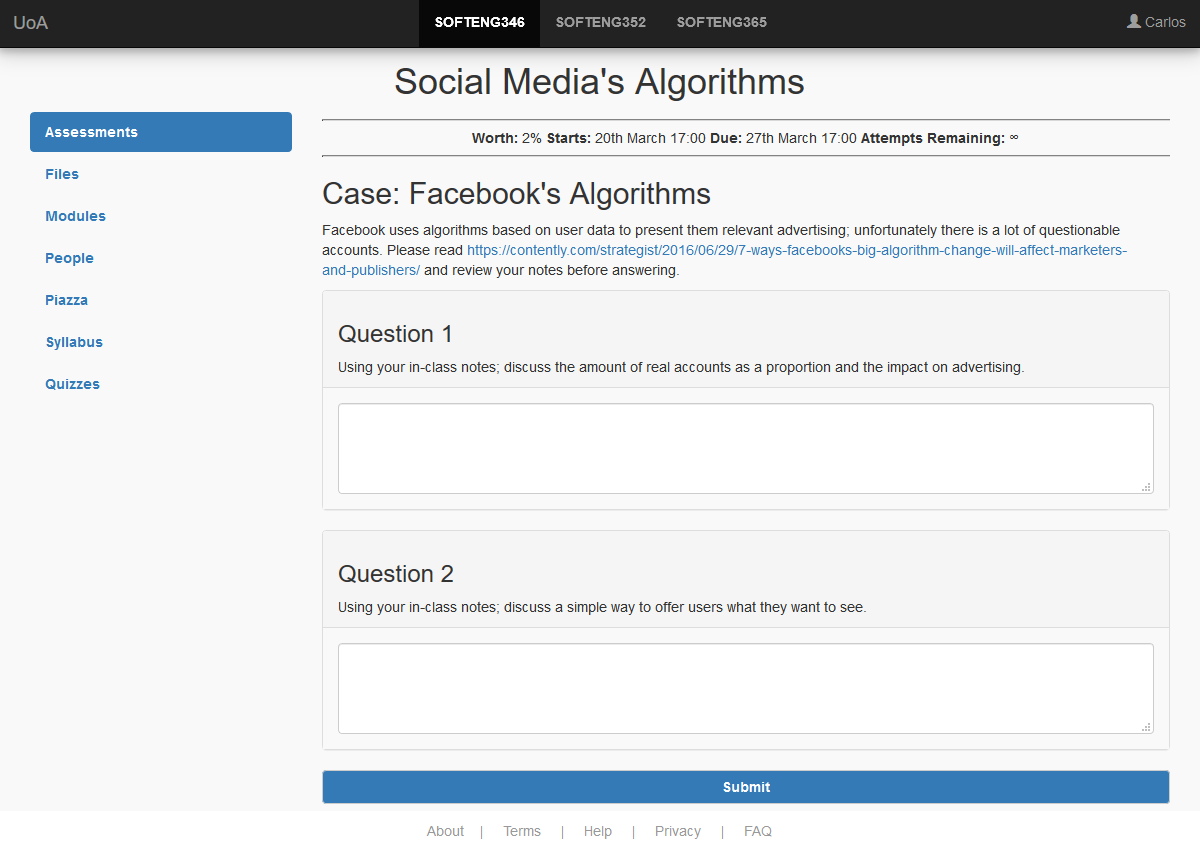
\includegraphics[width=\textwidth]{1 - Social Medias Algorithms.PNG}
		\caption{filling in the case with structured questions}
		\label{fig:one}
	\end{figure}
	\begin{figure}[H]
		\centering
		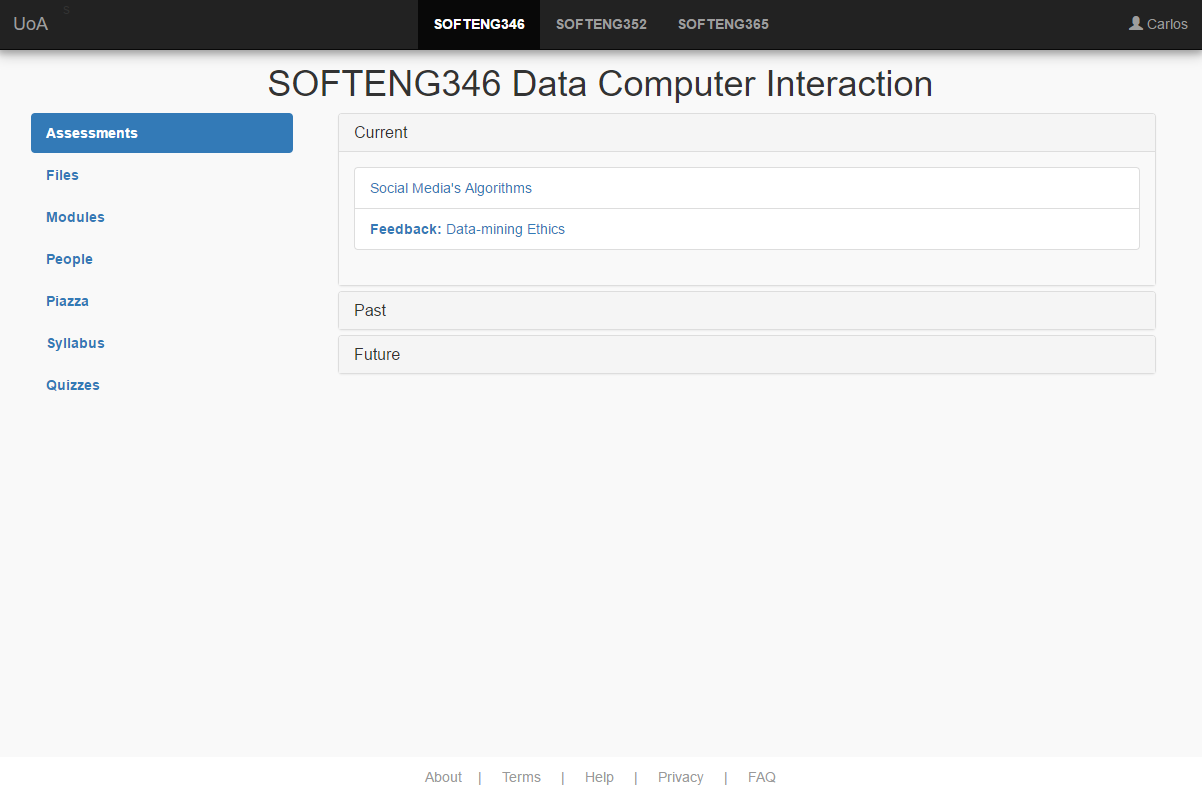
\includegraphics[width=\textwidth]{2 - Assessments (Current).PNG}
		\caption{list of assignments; specifically the current ones}
		\label{fig:two}
	\end{figure}
	\begin{figure}[H]
		\centering
		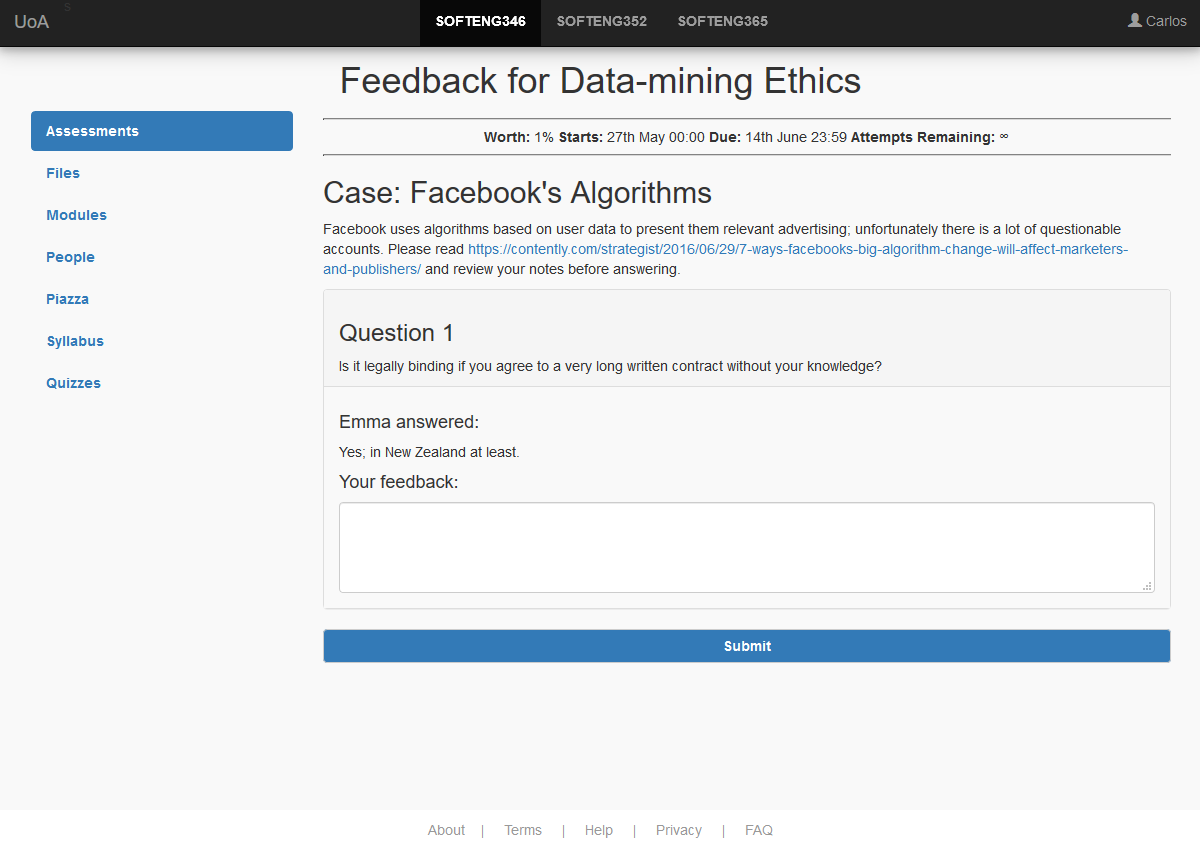
\includegraphics[width=\textwidth]{3 - Feedback for Data-mining Ethics.PNG}
		\caption{filling in feedback for another class peer}
		\label{fig:three}
	\end{figure}
	\begin{figure}[H]
		\centering
		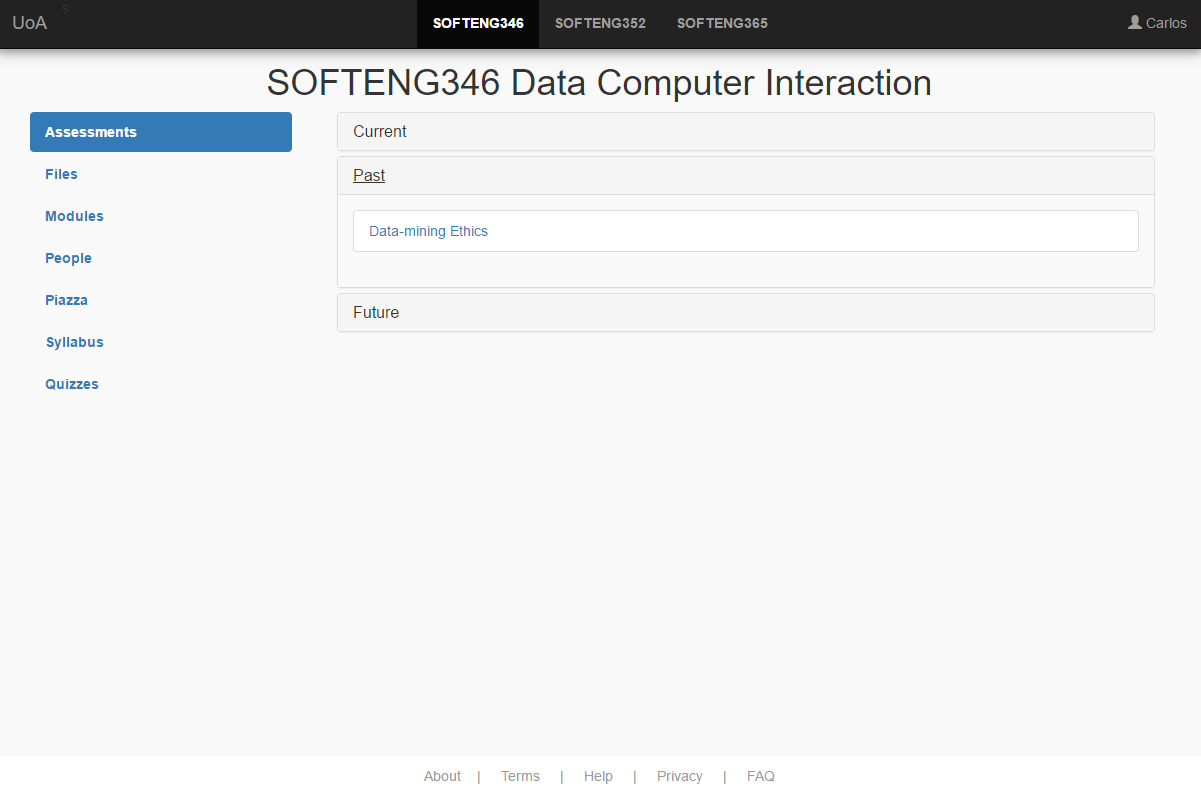
\includegraphics[width=\textwidth]{4 - Assessments (Past).PNG}
		\caption{list of assignments; specifically the previously submitted ones}
		\label{fig:four}
	\end{figure}
	\begin{figure}[H]
		\centering
		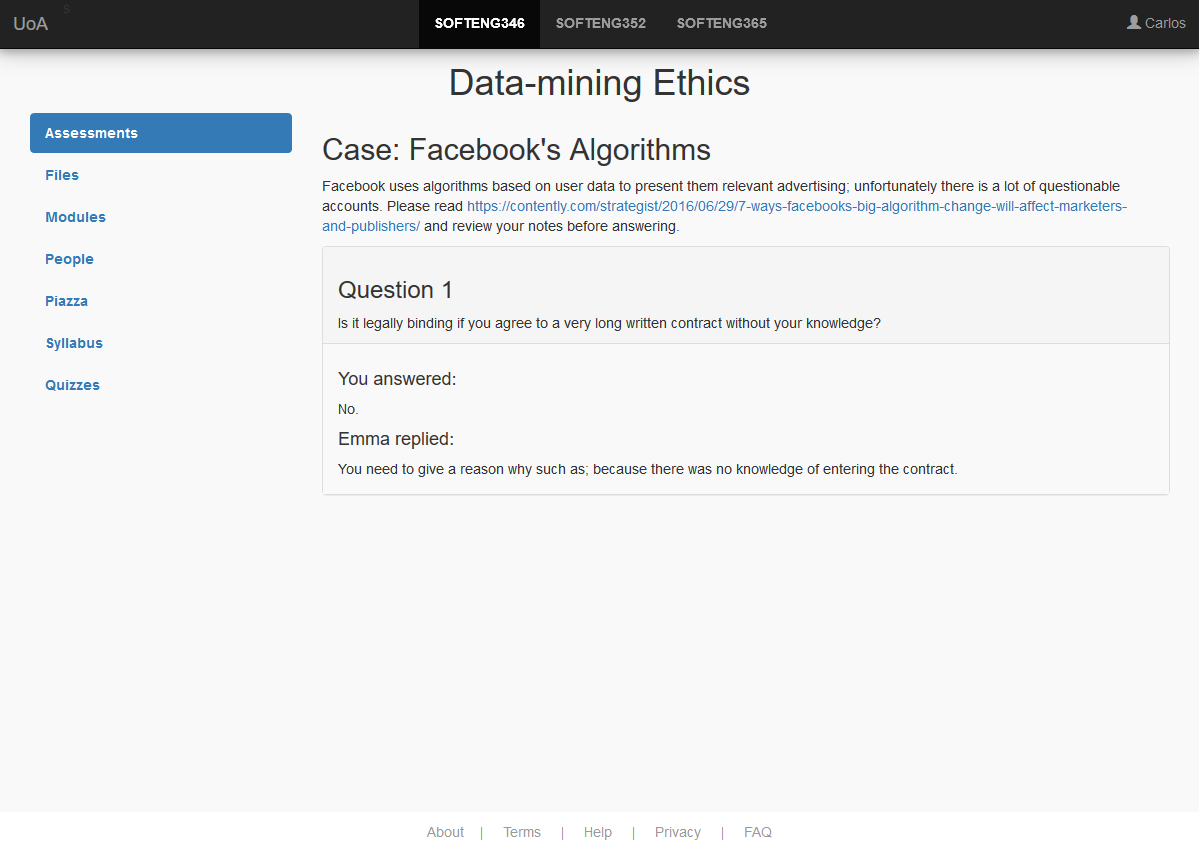
\includegraphics[width=\textwidth]{5 - Data-mining Ethics.PNG}
		\caption{reviewing another peer's feedback to the user}
		\label{fig:five}
	\end{figure}





	200-600words
	\subsection*{UI not implemented}
		list features that you thought you couldnt do
		-remembering stuff to be saved in fields
	\subsection*{UI implemented}
		\begin{itemize}
			\item other courses (SE364, SE351, EG303)
			\item personal settings
			\item home/home button
			\item footer links
		\end{itemize}
\section{Colour Scheme}
	50-200
	TALK ABOUT INPUT TEXT
	TALK ABOUT HIGHLIGHTING WITh CLICK OR TAB
	\begin{itemize}
		\item slightly off white backgound
		\item white nav text, black bar, slightly less black active, grey glypicon
		\item white footer
		\item black submission details
		\item blue side bar with white text bolded
		\item footer text color
		\item hover colour (white on navbar, darker on pill text and button)
		\item active colour (white on navbar text, darker navbar box, blue pill and white text for pills)
		\item submit button and text
		\item accordion container, group,panel,body,list,badges
		\item Question group, heading, group, header, answer box, 
	\end{itemize}
\section{Borders Scheme}
	100-250
	\begin{itemize}
		\item the horizontal rules around the submission details
		\item footer to main
		\item nav to header
		\item header to main
		\item sidebar to content
		\item | between the footer items
	%	\item box-shadow\: 0 4px 8px 0 rgba(0, 0, 0, 0.2), 0 6px 20px 0 rgba(0, 0, 0, 0.19); from \url{https://www.w3schools.com/css/css3_shadows.asp}
	\end{itemize}
\section{Fonts Scheme}
	100-250
	\begin{itemize}
		\item assignment submission details
		\item bolded categories
		\item bolded subject
		\item more bolding? what is not?
		\item 3 fonts of nav
		\item font of categories
		\item font of content.....
		\item font of footer
	\end{itemize}
\section{Resources Used}
	\subsection*{bootstrap}
		\begin{itemize}
			\item nawbar
			\item person glyphicon
			\item search for glyphicons
			\item look at classes (go through with a class equals "
		\end{itemize}
\end{document}
%https://piazza.com/class/iw7ylbqrrti7i?cid=243
%https://piazza.com/class/iw7ylbqrrti7i?cid=240
%user interacts with answer boxes to make them bigger